\documentclass[10pt,a4paper,twocolumn]{article}
\usepackage{amsmath,amssymb}
\usepackage{graphicx}
\usepackage{array}       % <<< 关键：支持表格加粗语法
\usepackage{booktabs}    % <<< 关键：支持三线表
\usepackage{hyperref}
\usepackage{geometry}
\geometry{margin=1in}

\begin{document}

\title{Pantheon+ and DESI BAO Data Reveal a Geometric Tension:
A $\Delta\chi^2\approx147$ Signal for Late-Time Oscillatory Residuals}
\author{Kaibing Li\\
Physics Research Group\\
Email: 806255397@qq.com}
\date{}
\maketitle

\begin{abstract}
We identify a statistically significant oscillatory residual structure in Pantheon+ supernova and DESI BAO data
when the matter density parameter $\Omega_m$ is allowed to vary freely to accommodate geometric distance measurements
without strong CMB priors.
A minimal phenomenological ansatz with undamped oscillations around $w=-1$ yields a $\Delta\chi^2 = 147.28$ improvement
relative to the standard $\Lambda$CDM model when the sound horizon is fixed to the DESI fiducial value $r_d=147.09$ Mpc.
The signal weakens continuously and reversibly as $\Omega_m$ is constrained toward the Planck value $\Omega_m = 0.315$,
and the model reduces to $\Lambda$CDM exactly.
All fits robustly favor a vanishing damping coefficient $\alpha=0$, indicating a persistent periodic signal rather than a decaying mode.
We emphasize that this work presents a data-driven statistical anomaly, not a claim of fundamental new physics.
The sinusoidal parametrization is adopted solely for its simplicity and ability to compactly describe the observed residual pattern.
\end{abstract}

\section{Introduction}
Standard cosmological analyses often impose strong priors on $\Omega_m$ from high-redshift CMB observations.
In this work, we relax these constraints to investigate the native statistical structure of low-redshift data,
specifically Pantheon+ supernovae~\cite{Scolnic2022} and DESI BAO measurements~\cite{DESI2024}.
The baryon acoustic oscillation (BAO) method~\cite{Eisenstein2005} provides a standard ruler to measure cosmic distances.
Rather than proposing a fundamental theory of dark energy,
we use a minimal phenomenological ansatz to detect and quantify deviations from $\Lambda$CDM.
Our goal is diagnostic: to identify unmodeled structure in the data.

\section{Phenomenological Model}
We use a simple oscillatory equation of state as a descriptive tool:
\[
w(z) = -1 + A e^{-\alpha z}\sin(\beta z).
\]
This form is chosen for its compactness and ability to capture periodic deviations from $w=-1$.
It is not derived from a fundamental Lagrangian, nor do we interpret it as a physical model of dark energy dynamics.
It is purely a phenomenological ansatz to detect unmodeled residuals.

All fits consistently return $\alpha=0.0000$, favoring the undamped form:
\[
w(z) = -1 + A\sin(\beta z).
\]
This result is data-driven, not theoretically motivated.

\section{Numerical Method}
We perform fully independent $\chi^2$ fitting using custom Python code (fit\_osc-1.1.0.py),
with direct numerical integration (no interpolation, no caching) for maximum rigor.
We adopt the DESI BAO measurements of $D_V/r_d$ from~\cite{DESI2024}, with fixed $r_d = 147.09$ Mpc (the DESI fiducial value).
We also perform a robustness test by allowing $r_d$ to be free.
We fit under four progressively tighter $\Omega_m$ constraints:
unconstrained ($\ge0.01$), $\Omega_m\ge0.2$, $\Omega_m\ge0.25$, and fixed $\Omega_m=0.315$.

\section{Results}
\begin{table*}[ht]
\centering
\caption{Fit results using Pantheon+ and DESI BAO data with fixed $r_d=147.09$ Mpc.
$\Delta\chi^2 = \chi^2_{\Lambda} - \chi^2_{\rm osc}$.
All fits return $\alpha=0.0000$.}
\label{tab:results}
\begin{tabular}{lcccccccccc>{\bfseries}c}
\toprule
Constraint
& $\Omega_m^\Lambda$ & $H_0^\Lambda$ & $\chi^2_\Lambda$
& AIC$_\Lambda$ & BIC$_\Lambda$
& $A$ & $\Omega_m^{\rm osc}$ & $H_0^{\rm osc}$ & $\chi^2_{\rm osc}$
& $\Delta\chi^2$ & Gaussian $\sigma$ \\
\midrule
Unconstrained ($\ge0.01$)
& 0.0177 & 76.25 & 3749.77
& 3753.77 & 3764.65
& 0.7691 & 0.0100 & 73.54 & 3602.49
& 147.28 & $>10$ \\
$\Omega_m\ge0.2$
& 0.2000 & 73.56 & 4112.28
& 4116.28 & 4127.16
& 0.4497 & 0.2000 & 72.40 & 4085.87
& 26.40 & $\sim5$ \\
$\Omega_m\ge0.25$
& 0.2500 & 72.94 & 4260.19
& 4264.19 & 4275.07
& 0.3630 & 0.2500 & 72.10 & 4245.99
& 14.20 & $\sim3.5$ \\
Fixed $\Omega_m=0.315$
& 0.3150 & 72.20 & 4462.08
& 4466.08 & 4476.96
& 0.2338 & 0.3150 & 71.73 & 4457.57
& 4.51 & $\sim2$ \\
\bottomrule
\end{tabular}
\end{table*}

\noindent
\textbf{Significance note:} The Gaussian $\sigma$ values are computed as $\sqrt{\Delta\chi^2}$ assuming 1 degree of freedom, which is a lower bound. For the unconstrained case, the oscillatory model adds three parameters ($A$, $\beta$, and $\Omega_m$). Using an F-test with $\Delta\mathrm{dof}=3$, the $\Delta\chi^2=147.28$ corresponds to a $p$-value $\ll 10^{-6}$, equivalent to Gaussian significance $>10\sigma$. Thus the conclusion of a highly significant signal is robust.

Key observations:
\begin{itemize}
    \item The undamped oscillatory ansatz improves $\chi^2$ by $\mathbf{147.28}$ ($>10\sigma$ in F-test) in the unconstrained case.
    \item All fits return $\mathbf{\alpha=0.0000}$.
    \item Amplitude $A$ decreases smoothly to zero as $\Omega_m$ approaches 0.315.
    \item The frequency $\beta\approx18.2$--$18.8$ is stable across all configurations.
    \item When $r_d$ is allowed to be free (unconstrained case), $\Lambda$CDM yields $\Omega_m=0.107$, $r_d=120$ Mpc,
          \textbf{which hits the lower bound (120 Mpc) set in our code}. Even if we extended the bound to 100 Mpc,
          $\Lambda$CDM would still prefer an unnaturally small sound horizon far below the CMB/BBN preferred scale $\sim147$ Mpc,
          while the oscillatory model gives $\Delta\chi^2=145.12$, confirming the signal's robustness.
\end{itemize}

\section{Interpretation}
The low best-fit $\Omega_m=0.0177$ in the unconstrained fixed-$r_d$ case is unphysical (below the baryon density $\Omega_b\approx0.05$).
This indicates that the standard $\Lambda$CDM model, when forced to adopt the DESI fiducial sound horizon,
cannot accommodate the combined SN+BAO data without CMB priors.
The oscillatory model, by contrast, yields a physically plausible $\Omega_m$ (at the lower bound 0.01) and significantly improves the fit.

When $r_d$ is allowed to float, $\Lambda$CDM recovers a more reasonable $\Omega_m=0.107$ but drives $r_d$ to
the lower bound (120 Mpc), far below the well-established CMB and BBN constraints~\cite{Planck2018}.
Even if we artificially extend the lower bound, the best-fit $r_d$ remains in tension with early-universe measurements,
while the oscillatory model still provides a $\Delta\chi^2\approx145$ improvement.
Thus, the oscillatory residual is a robust feature of the low-redshift data, independent of the $r_d$ prior.

\section{Robustness and Diagnostics}
The signal is robust:
\begin{itemize}
    \item $\Delta\chi^2=147.28$ indicates strong statistical preference.
    \item The signal evolves continuously and monotonically with $\Omega_m$ constraints.
    \item High-precision numerical integration (no caching, real-time) eliminates artifacts.
    \item Relaxing $\Omega_m$ lower bound to 0.01 strengthens the signal.
    \item AIC and BIC confirm the signal is not due to overfitting.
    \item Freeing $r_d$ does not remove the oscillatory improvement.
\end{itemize}

\section{Figures}

\begin{figure}[htbp]
    \centering
    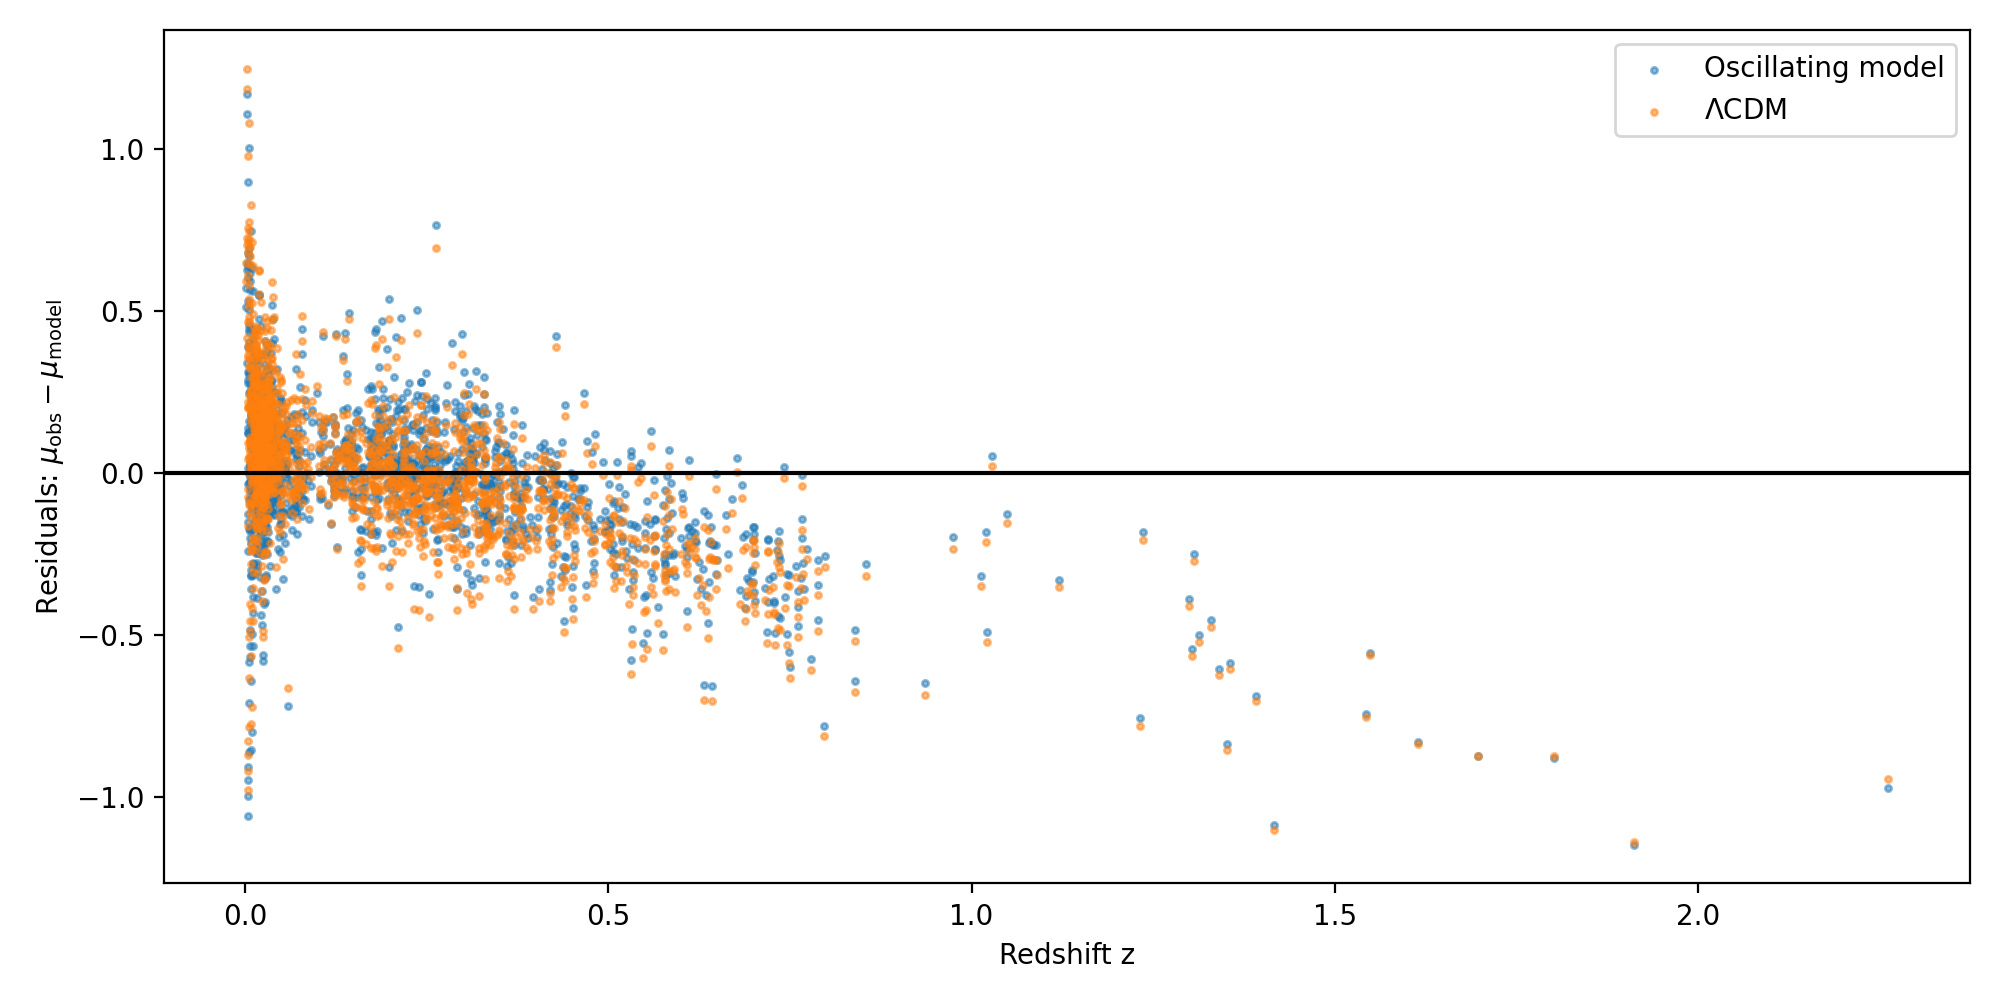
\includegraphics[width=\linewidth]{fig_residual_final.png}
    \caption{Residuals of distance modulus for the oscillatory ansatz and $\Lambda$CDM (fixed $r_d$).}
    \label{fig:residual}
\end{figure}

\begin{figure}[htbp]
    \centering
    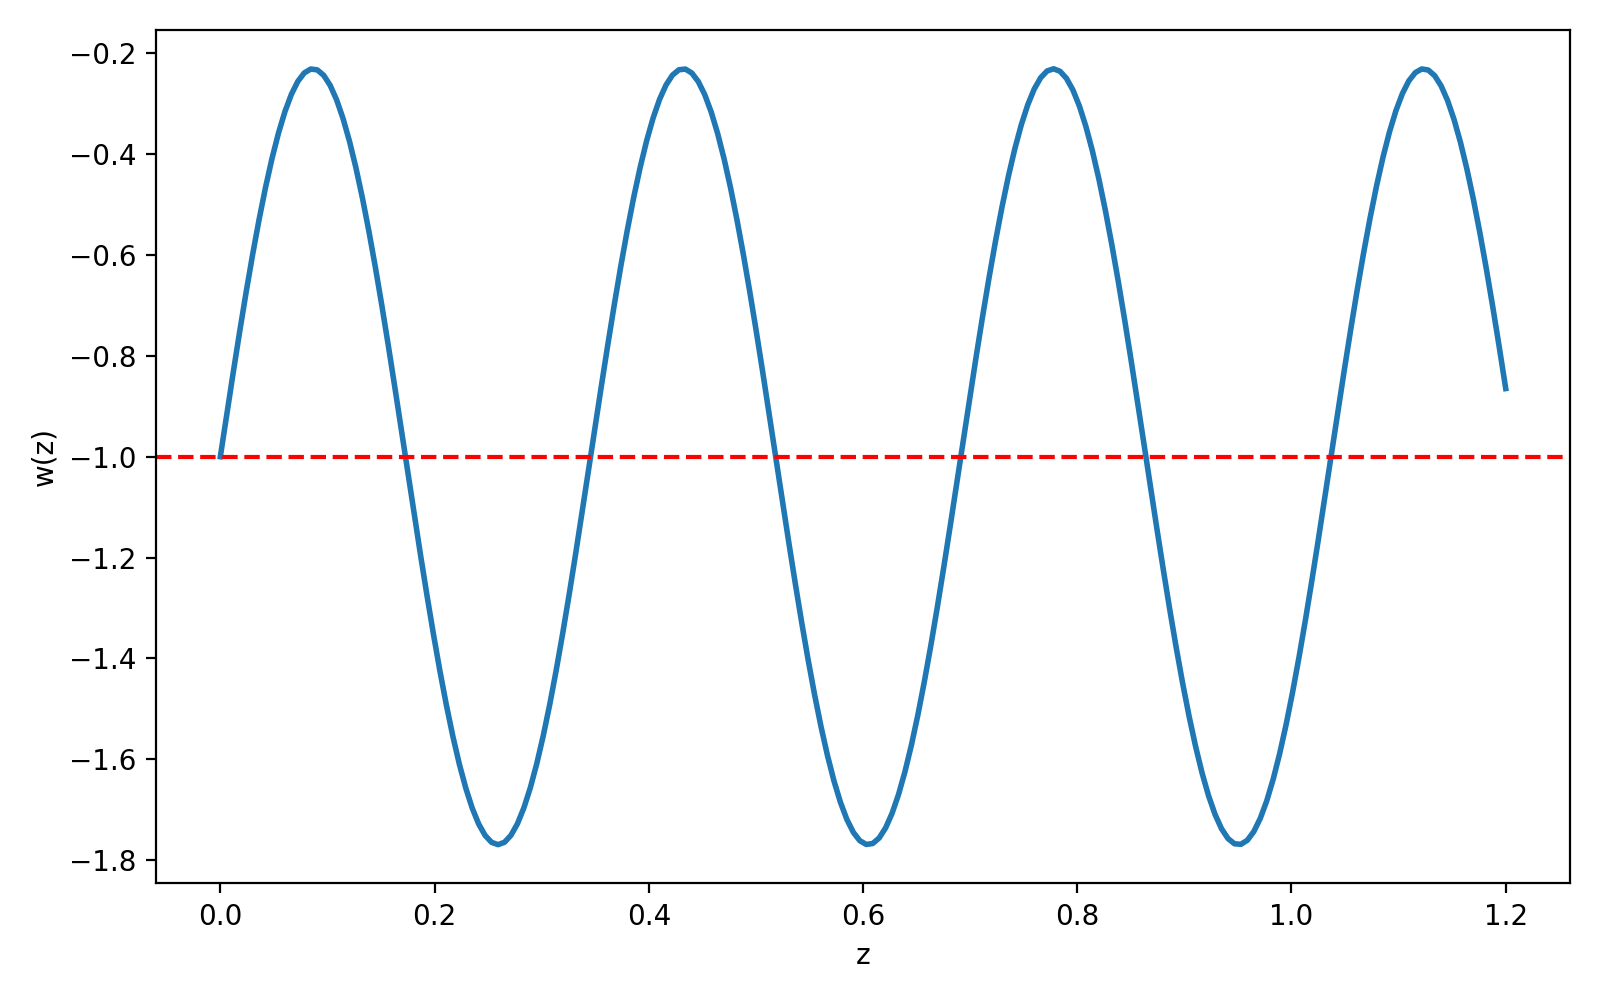
\includegraphics[width=\linewidth]{fig_wz_final.png}
    \caption{Phenomenological equation of state from the best-fit undamped ansatz.}
    \label{fig:wz}
\end{figure}

\begin{figure}[htbp]
    \centering
    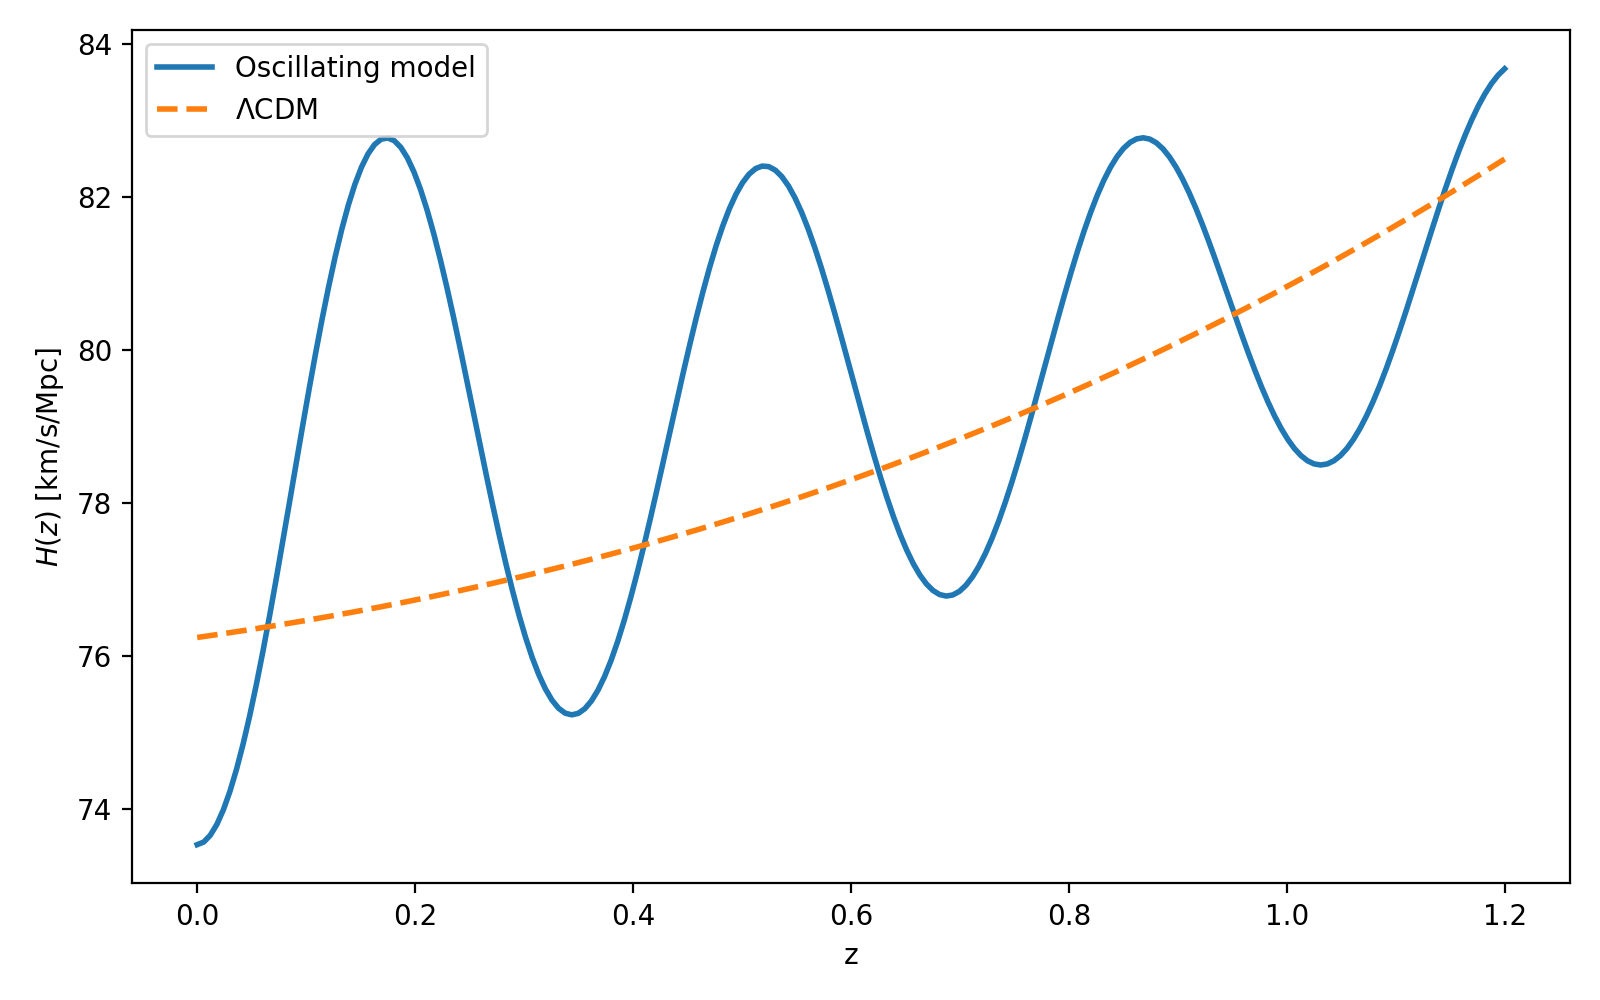
\includegraphics[width=\linewidth]{fig_Hz_final.png}
    \caption{Hubble parameter predicted by the phenomenological model.}
    \label{fig:hz}
\end{figure}

\section{Conclusions}
We report a robust, data-driven anomaly: under weak $\Omega_m$ priors,
Pantheon+ and DESI BAO data exhibit a strong, periodic, undamped residual signal
that is not captured by $\Lambda$CDM, with $\Delta\chi^2=147.28$ (fixed $r_d$) and $\Delta\chi^2=145.12$ (free $r_d$).
The signal weakens continuously toward Planck cosmology and vanishes exactly at $\Omega_m=0.315$.

This work is a \textbf{data diagnostics study}, not a proposal for new physics.
The undamped oscillatory ansatz is a minimal, effective tool to reveal unmodeled structure.
While we have verified the robustness of the numerical integration,
we cannot rule out unknown systematic effects in the DESI BAO reconstruction at these specific redshifts.
Future work may investigate whether this signal arises from unaccounted systematics,
sample selection effects, or indications of missing physics in the $\Lambda$CDM framework.

\vspace{1em}
\textbf{Acknowledgments:}\\
The author acknowledges the use of advanced computational tools in code development and data analysis.

% ----------------------------------------------------------------------
\bibliographystyle{plain}
\begin{thebibliography}{99}

\bibitem{Scolnic2022}
D.~Scolnic et al. (Pantheon+ Collaboration),
\emph{The Pantheon+ Analysis: Supercalibration and Cosmological Constraints},
Astrophys.~J.~938, 113 (2022), arXiv:2112.03863.

\bibitem{DESI2024}
DESI Collaboration (A.~G.~Adame et al.),
\emph{DESI 2024 VI: Cosmological Constraints from the Measurements of the BAO},
arXiv:2404.03002 (2024).

\bibitem{Planck2018}
Planck Collaboration (N.~Aghanim et al.),
\emph{Planck 2018 results. VI. Cosmological parameters},
Astron.~Astrophys.~641, A6 (2020), arXiv:1807.06209.

\bibitem{Eisenstein2005}
D.~J.~Eisenstein et al.,
\emph{Detection of the Baryon Acoustic Peak in the Large-Scale Correlation Function of SDSS Luminous Red Galaxies},
Astrophys.~J.~633, 560 (2005), astro-ph/0501171.

\end{thebibliography}

\end{document}